\begin{enumerate}[label=\thesubsection.\arabic*.,ref=\thesubsection.\theenumi]
\numberwithin{equation}{enumi}
\item
Sketch the Polar Plot of
\begin{align}
G\brak{s} = \frac{1}{s\brak{1+s^{2}}}
\label{eq:ee18btech11023_gain}
\end{align}
\\
\solution  From \eqref{eq:ee18btech11023_gain},

\begin{align}
G\brak{\j\omega} &=   \frac{1}{\j\omega\brak{1-{\omega}^{2}}}
\\
      \abs{G\brak{\j\omega}} &= \frac{1}{\abs{\omega\brak{1-{\omega}^{2}}}}
\\
    \angle G\brak{\j\omega} &= 
\begin{cases}
\frac{\pi}{2} & \omega > 1
\\
-\frac{\pi}{2} & 0 < \omega < 1
\end{cases}
    \end{align}
%
The corresponding polar plot is generated in Fig.   \ref{fig:ee18btech11023} using 
\begin{lstlisting}
codes/ee18btech11023.py
\end{lstlisting}

\begin{figure}[!ht]
\centering
  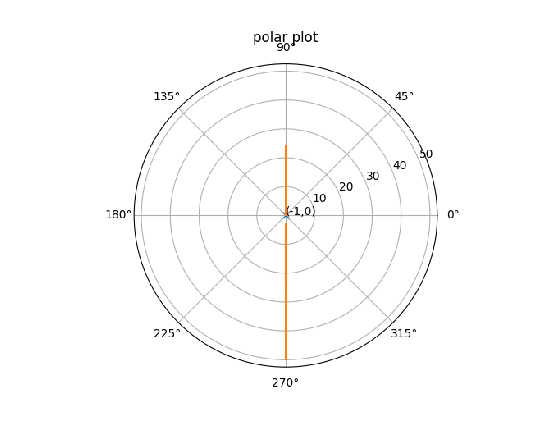
\includegraphics[width=\columnwidth]{./figs/ee18btech11023/ee18btech11023_1c.eps}
  \caption{}
  \label{fig:ee18btech11023}
\end{figure}
In Fig.   \ref{fig:ee18btech11023},  (–1,0) is exactly on the polar plot.  Hence, the system is marginally stable.


\end{enumerate}
